\documentclass{article}

\usepackage[utf8x]{inputenc}
\usepackage{ucs}
\usepackage{amsmath}
\usepackage{amsfonts}
\usepackage{amssymb}
\usepackage{mathtools}
\usepackage{color}
\usepackage{xcolor}
\usepackage{listings}
\usepackage{url}
\usepackage{graphicx,xspace}
\usepackage{float}

\usepackage[margin=1in]{geometry}

\usepackage{titling}
\setlength{\droptitle}{-1in}

\usepackage[margin=1in]{caption}  

\usepackage{courier}

\newcommand{\sudo}{\texttt{sudo}\xspace}

\lstset{%
 xleftmargin=0cm,
 stepnumber=1,
 %numbers=left,
 numbersep=5pt,
 numberstyle=\ttfamily\tiny\color[gray]{0.3},
 belowcaptionskip=\bigskipamount,
 captionpos=b,
 escapeinside={@}{@},
 tabsize=2,
 emphstyle={\tt},
 commentstyle=\it,
 stringstyle=\ttfamily\small,
 showspaces=false,
 keywordstyle=\bfseries,
 morekeywords={if, input, print}, 
 columns=flexible,
 basicstyle=\ttfamily,%\small,
 showstringspaces=false,
 morecomment=[l]\%,
 backgroundcolor = \color{lightgray},
 framexleftmargin = 1em
}

\setlength{\parindent}{0.2in}

\title{System Administration, Machines, Users, and Groups\vspace{-2ex}}
\author{Annie Christy}
\date{}

\begin{document}

\maketitle

\section*{What is System Administration?}

System administrators set up and maintain computer systems. We put hard drives
into machines, plug machines into walls, install operating systems, monitor and
assemble networks, install and upgrade software, manage user accounts and
permissions,  guard secure information, log system actions, store system
backups, provide web and email services, and troubleshoot any issues that arise
on the system. We will be covering most of these topics in this class, although
much of the setup (like plugging in the computer and installing operating
systems) has been done for you. The labs will begin with basic Unix/Linux
concepts and progress toward the configuration of more complicated services. You
will mostly be dealing with client-side configuration, but if you are
interested, we encourage you to learn more about setting up the services on your
own personal machines.

\section*{Honor Code} The techniques and commands that you will learn in this
class are powerful and important to a system administrator. However, you always
need to be aware of what you are allowed to do on the system you are working on.
We have given you extra root privileges and access to the machines that were set
up specifically for this course. Don't abuse those privileges. 
Just because you \textit{can} access information doesn't mean you \textit{should}.
\\

\noindent Before you start working, you should read the CS Department's
acceptable use policy. All of it.

\vspace{1em}

\url{http://www.cs.hmc.edu/wiki/QREF/Policy}

\vspace{1em}

\noindent\textbf{Always ask yourself if it's technically necessary and 
ethically justified to use your sysadmin priviledges and knowledge.}


% \section*{Where to Find Help}
% -grutors?\\
% -in class tutoring?\\
% -prof ben?\\
% -policy on googling solutions?\\
% -NOT THE REQUEST SYSTEM!!!\\

% \section*{Grading}
% -how the class will be graded\\
% -what a completed assignment looks like\\
% -participation\\
% -additional projects\\


\section*{The System Administration Machines}

The system you will be working with in this class is modeled off the cluster
that the Computer Science department uses. Most of the departmental machines run
the Gentoo operating system, so that is what we will be using as well.
Currently, we have three machines that have been set up for this course. Crispy
is the name of our main server. It hosts the services that you will be using for the duration
of the class. Gred and Forge host the virtual machines that you will be working
with.

\section*{Meet Your (Virtual) Machine} 
You will get your own viritual machine to administer during the semester.
Information on how to access your machines will be provided in lab.

\section*{Users}

When you first log into your machine, you should see a command prompt ending in
a pound sign. Although the appearance of the prompt can be changed, a pound sign
traditionally denotes a root prompt. Root users have access to everything on the
machine. For this reason, it is a bad idea to spend a lot of time working with a
root prompt because you could do something accidentally that you did not mean
to, the root account could be left open and vulnerable, and it is harder for
malicious applications to attack your system, among other reasons.

At this point, your computer has no users besides root. You can use the useradd
command to create an account for yourself. The command in the gray box below
will create the account for you. Remember to replace  $<$username$>$ with your
username (please use your knuth username). The -m flag tells the command to
create a home directory for you in /home. The -k flag tells useradd to populate
that directory with the contents of the /etc/skel directory which has been
provided for you. the -G flag tells the command to add the user to the groups
that are specified in the comma-separated list that follows it. The -s option
tells the command to use /bin/bash as the default shell. Finally, you specify
the username.

\begin{lstlisting}[language = bash]
useradd -m -k /etc/skel -G users,wheel,portage -s /bin/bash <username>
\end{lstlisting}

Next, you need to create a password for your account. Use the passwd command
then enter your password when you are prompted to.

\begin{lstlisting}[language = bash]
passwd <username>
\end{lstlisting}

Now log out of your machine...

\begin{lstlisting}[language = bash]
exit
\end{lstlisting}

...and log back in using the account you just created. \\\\

Find a buddy and create an account for him or her on your machine.\footnote{You'll 
probably have to use the full path of the command to add add a user: 
\texttt{/usr/sbin/useradd}} Don't give
them root access though; the two of you aren't that close. Note that you are no
longer working from a root account, so you don't actually have permission to
create a user. However, you have superuser access on your machine (since you are
in the wheel group) so you can still run the command if you append it with the
word \sudo. Once the accounts are set up, try remotely logging into each other's machines
using the new accounts.

\section*{Groups}

Linux systems use a mechanism called \textit{groups} to  cluster users into access
groups. It is possible for certain files and applications to be set as readable,
writable or executable only by users in a particular group. In this way, a
system administrator can give some users access to applications that they don't
trust others to use.

Some important groups that come with a standard Gentoo installation include:

\begin{tabular}{|c|c|}
\hline
Group & Purpose \\
\hline
audio & access to audio devices  \\
cdrom & access to optical devices \\
floppy & access to floppy devices \\
games & ability to play games \\
portage & ability to run a pretend emerge \\
usb & access to USB devices \\
video & access to video hardware \\
wheel & superuser abilities \\
 \hline
\end{tabular}\\ \\


You can view the groups you are assigned to with the groups command.

\begin{lstlisting}[language = bash]
groups
\end{lstlisting}

You should be in the wheel, users, and portage groups. You will also be in a
group that is the same as your username. The wheel group is probably the most
important group to be aware of for the purposes of this class. Since you are in
this group, you can use the \sudo command along with your account password to run
commands as a superuser. System administrators do this a lot because most
actions that will drastically change your computer or your system need an
administrator's permission to execute. You will be doing more with group
permissions and superuser commands in the next lab.\\

It is also possible to create new groups on your system. This is done using the
groupadd command. Create a group called \texttt{friends}.

\begin{lstlisting}[language = bash]
sudo groupadd friends
\end{lstlisting}

Add yourself to the newly created group with the usermod command.

\begin{lstlisting}[language = bash]
sudo usermod -a -G friends <username>
\end{lstlisting}

Add your buddy to the group as well. \\

Now, if you log into each other's machines, and type \texttt{groups}, you will be in each
other's friends group! Great job. I'm so proud.\\

Unfortunately, you and your buddy had a big fight, and you don't want him/her to
use your computer anymore. You can delete a user account with the userdel
command. The -r flag tells the machine to delete their home directory as well so
you don't have to deal with all of the stuff they left on your computer after
you kick them out. Delete your buddy's account now.

\begin{lstlisting}[language = bash]
userdel -r <buddy>
\end{lstlisting}
If you see the following error message, you can ignore it: 

\begin{lstlisting}[language = bash,backgroundcolor=\color{white}]
userdel: <buddy> mail spool (/var/spool/mail/<buddy>) not found
\end{lstlisting}

\begin{figure}[H]
\centering
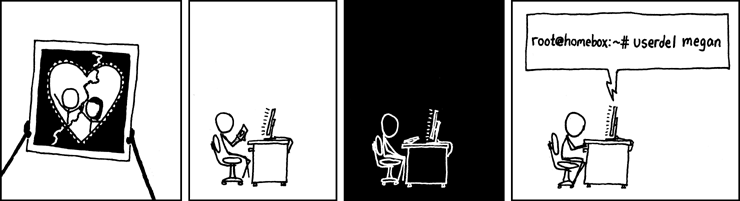
\includegraphics[width=.9\textwidth]{letting_go.png}
\caption{http://imgs.xkcd.com/comics/letting\_go.png}

\label{fig:letitgo}
\end{figure}


Great! Your machine is all set up. We hope you have a super fun and amazing
semester learning about system administration.\\

---CS Staff (Annie Christy, Jo\v{z}i McKiernan, Jeff Milling, Hu Lin, Paige Rinnert, Lisa
Goeller, Prof. Ben)

\section*{References}
\begin{verbatim}
http://superuser.com/questions/242294/what-is-purpose-of-etc-shadow-and-
        shadow-cache-files-in-linux-operating-system
http://www.cyberciti.biz/faq/understanding-etcpasswd-file-format/
http://www.cyberciti.biz/faq/understanding-etcgroup-file/
http://www.linuxquestions.org/questions/ubuntu-63/etc-gshadow-681676/
http://www.linfo.org/etc_skel.html
http://uw714doc.sco.com/en/SM_basics/etc_default_useradd.html
http://man7.org/linux/man-pages/man5/login.defs.5.html
http://forums.gentoo.org/viewtopic-t-805507-start-0.html
https://www.gentoo.org/doc/en/handbook/handbook-x86.xml?part=1&chap=11
http://xkcd.com/215/
\end{verbatim}


\end{document}




